% Options for packages loaded elsewhere
\PassOptionsToPackage{unicode}{hyperref}
\PassOptionsToPackage{hyphens}{url}
%
\documentclass[
  letterpaper,
  ignorenonframetext,
  aspectratio=43,
  handout,
  12pt]{beamer}
\usepackage{pgfpages}
\setbeamertemplate{caption}[numbered]
\setbeamertemplate{caption label separator}{: }
\setbeamercolor{caption name}{fg=normal text.fg}
\beamertemplatenavigationsymbolsempty
% Prevent slide breaks in the middle of a paragraph
\widowpenalties 1 10000
\raggedbottom
\setbeamertemplate{part page}{
  \centering
  \begin{beamercolorbox}[sep=16pt,center]{part title}
    \usebeamerfont{part title}\insertpart\par
  \end{beamercolorbox}
}
\setbeamertemplate{section page}{
  \centering
  \begin{beamercolorbox}[sep=12pt,center]{part title}
    \usebeamerfont{section title}\insertsection\par
  \end{beamercolorbox}
}
\setbeamertemplate{subsection page}{
  \centering
  \begin{beamercolorbox}[sep=8pt,center]{part title}
    \usebeamerfont{subsection title}\insertsubsection\par
  \end{beamercolorbox}
}
\AtBeginPart{
  \frame{\partpage}
}
\AtBeginSection{
  \ifbibliography
  \else
    \frame{\sectionpage}
  \fi
}
\AtBeginSubsection{
  \frame{\subsectionpage}
}
\usepackage{amsmath,amssymb}
\usepackage{lmodern}
\usepackage{ifxetex,ifluatex}
\ifnum 0\ifxetex 1\fi\ifluatex 1\fi=0 % if pdftex
  \usepackage[T1]{fontenc}
  \usepackage[utf8]{inputenc}
  \usepackage{textcomp} % provide euro and other symbols
\else % if luatex or xetex
  \usepackage{unicode-math}
  \defaultfontfeatures{Scale=MatchLowercase}
  \defaultfontfeatures[\rmfamily]{Ligatures=TeX,Scale=1}
\fi
\usetheme[]{metropolis}
% Use upquote if available, for straight quotes in verbatim environments
\IfFileExists{upquote.sty}{\usepackage{upquote}}{}
\IfFileExists{microtype.sty}{% use microtype if available
  \usepackage[]{microtype}
  \UseMicrotypeSet[protrusion]{basicmath} % disable protrusion for tt fonts
}{}
\makeatletter
\@ifundefined{KOMAClassName}{% if non-KOMA class
  \IfFileExists{parskip.sty}{%
    \usepackage{parskip}
  }{% else
    \setlength{\parindent}{0pt}
    \setlength{\parskip}{6pt plus 2pt minus 1pt}}
}{% if KOMA class
  \KOMAoptions{parskip=half}}
\makeatother
\usepackage{xcolor}
\IfFileExists{xurl.sty}{\usepackage{xurl}}{} % add URL line breaks if available
\IfFileExists{bookmark.sty}{\usepackage{bookmark}}{\usepackage{hyperref}}
\hypersetup{
  hidelinks,
  pdfcreator={LaTeX via pandoc}}
\urlstyle{same} % disable monospaced font for URLs
\newif\ifbibliography
\usepackage{graphicx}
\makeatletter
\def\maxwidth{\ifdim\Gin@nat@width>\linewidth\linewidth\else\Gin@nat@width\fi}
\def\maxheight{\ifdim\Gin@nat@height>\textheight\textheight\else\Gin@nat@height\fi}
\makeatother
% Scale images if necessary, so that they will not overflow the page
% margins by default, and it is still possible to overwrite the defaults
% using explicit options in \includegraphics[width, height, ...]{}
\setkeys{Gin}{width=\maxwidth,height=\maxheight,keepaspectratio}
% Set default figure placement to htbp
\makeatletter
\def\fps@figure{htbp}
\makeatother
\setlength{\emergencystretch}{3em} % prevent overfull lines
\providecommand{\tightlist}{%
  \setlength{\itemsep}{0pt}\setlength{\parskip}{0pt}}
\setcounter{secnumdepth}{-\maxdimen} % remove section numbering
\usepackage{pgfpages}
\pgfpagesuselayout{2 on 1}
\providecommand{\tightlist}{%
\setlength{\itemsep}{0pt}\setlength{\parskip}{0pt}}
\makeatletter
\makeatother
\let\Oldincludegraphics\includegraphics
\renewcommand{\includegraphics}[2][]{\Oldincludegraphics[width=\textwidth,height=0.7\textheight,keepaspectratio]{#2}}
\ifluatex
  \usepackage{selnolig}  % disable illegal ligatures
\fi

\author{}
\date{}

\begin{document}

\begin{frame}{Mechanics of Materials}
\protect\hypertarget{mechanics-of-materials}{}
Lecture 3 - Strain

Dr.~Nicholas Smith

Wichita State University, Department of Aerospace Engineering

8 February, 2021
\end{frame}

\begin{frame}{schedule}
\protect\hypertarget{schedule}{}
\begin{itemize}
\tightlist
\item
  8 Feb - Strain, Homework 1 Due
\item
  10 Feb - Mechanical Properties
\item
  15 Feb - Exam Review, Homework 2 Due, Homework 1 Self-grade Due
\item
  17 Feb - Exam 1
\item
  19 Feb - Project 1 Due
\end{itemize}
\end{frame}

\begin{frame}{outline}
\protect\hypertarget{outline}{}
\begin{itemize}
\tightlist
\item
  allowable stress design
\item
  limit state design
\item
  strain
\end{itemize}
\end{frame}

\hypertarget{allowable-stress-design}{%
\section{allowable stress design}\label{allowable-stress-design}}

\begin{frame}{allowable stress}
\protect\hypertarget{allowable-stress}{}
\begin{itemize}
\tightlist
\item
  Most of the time, we design structures so the stress is less than some
  limit
\item
  By setting a conservative allowable stress, we account for some
  manufacturing tolerances, unintended loads, and variability in
  mechanical properties
\end{itemize}
\end{frame}

\begin{frame}{factor of safety}
\protect\hypertarget{factor-of-safety}{}
\begin{itemize}
\tightlist
\item
  The factor of safety is the failure load divided by the allowable load
\end{itemize}

\[FS = \frac{F_{fail}}{F_{allow}}\]

\begin{itemize}
\tightlist
\item
  Since load and stress are linearly proportional, we could also define
  the factor of safety in terms of stress and it would be identical
\end{itemize}
\end{frame}

\begin{frame}{factor of safety}
\protect\hypertarget{factor-of-safety-1}{}
\begin{itemize}
\item
  Typical values for the factor of safety will vary based on application
\item
  Aircraft and space vehicles might have a factor close to 1 to minimize
  weight
\item
  Nuclear power plants might have a factor close to 3 since weight is
  not as important and failure would be catastrophic
\end{itemize}
\end{frame}

\begin{frame}{simple connections}
\protect\hypertarget{simple-connections}{}
\begin{itemize}
\tightlist
\item
  We can rearrange the equations \(\sigma=N/A\) and \(\tau=V/A\) to size
  components based on some allowable stress
\end{itemize}

\[\begin{aligned}
  A &= \frac{N}{\sigma_{allow}}\\
  A &= \frac{V}{\tau_{allow}}
\end{aligned}\]
\end{frame}

\begin{frame}{bearing stress}
\protect\hypertarget{bearing-stress}{}
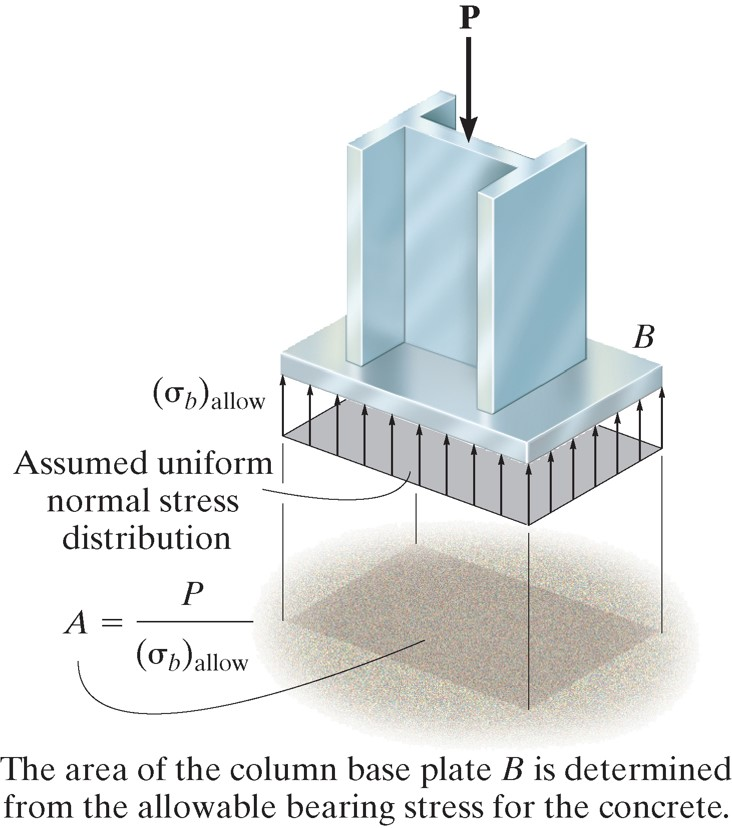
\includegraphics{../images/bearing-stress.jpg}
\end{frame}

\begin{frame}{embedded shear stress}
\protect\hypertarget{embedded-shear-stress}{}
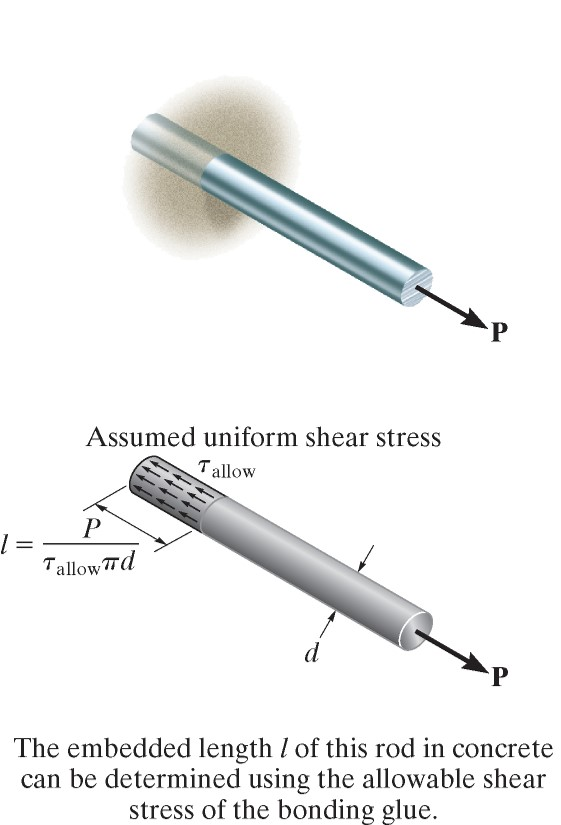
\includegraphics{../images/embedded-shear.jpg}
\end{frame}

\begin{frame}{lap joint shear}
\protect\hypertarget{lap-joint-shear}{}
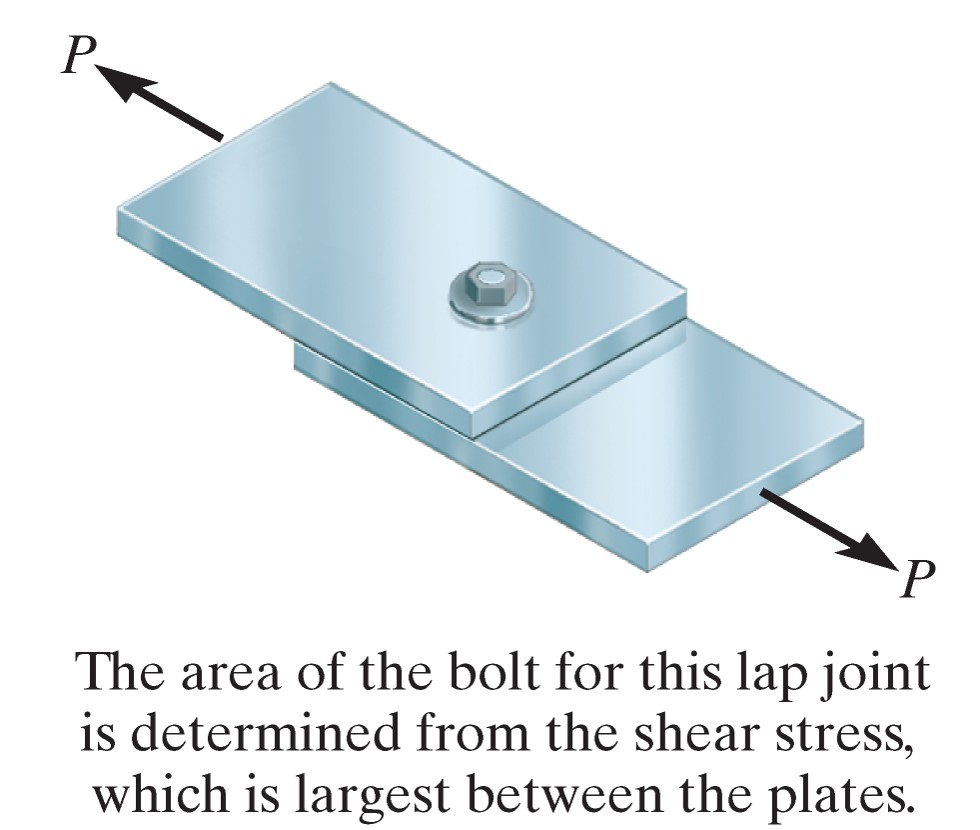
\includegraphics{../images/lap-shear.jpg}
\end{frame}

\hypertarget{limit-state-design}{%
\section{limit state design}\label{limit-state-design}}

\begin{frame}{limit state design}
\protect\hypertarget{limit-state-design-1}{}
\begin{itemize}
\tightlist
\item
  Allowable stress design accounts for uncertainty in the applied
  loading and the material properties in one factor of safety
\item
  Limit state design separates these two into load and resistance
  factors
\end{itemize}
\end{frame}

\begin{frame}{load factors}
\protect\hypertarget{load-factors}{}
\begin{itemize}
\tightlist
\item
  The load factor combines uncertainty in various types of load
\item
  For example, a building can have loading from a few different sources,
  such as its own weight, people in the building, and snow on top of the
  building
\item
  Weight is considered a \emph{dead load} and can usually be determined
  more precisely than moving things like people
\end{itemize}
\end{frame}

\begin{frame}{load factors}
\protect\hypertarget{load-factors-1}{}
\begin{itemize}
\item
  In this simple example, we consider a load factor, \(\gamma_D=1.2\)
  for the dead load, \(\gamma_L=1.6\) and \(\gamma_S=0.5\)
  \[R = 1.2D + 1.6L + 0.5S\]
\item
  These load factors combine the concept of a safety factor with the
  probability that loads will occur
\end{itemize}
\end{frame}

\begin{frame}{resistance factors}
\protect\hypertarget{resistance-factors}{}
\begin{itemize}
\item
  Resistance factors, \(\phi\) are used to express the probability a
  material will fail at its limit load
\item
  If we are very confident in the failure stress of a material (i.e.
  steel has little variability), we might use \(\phi=0.9\)
\item
  If we are not as confident, (using a new material, or an organic
  material like wood with higher variability), we might use \(\phi=0.7\)
\end{itemize}
\end{frame}

\begin{frame}{design criteria}
\protect\hypertarget{design-criteria}{}
\begin{itemize}
\tightlist
\item
  If we call the nominal load \(P\), then we can combine load and
  resistance factors using \[\phi P \ge R\]
\end{itemize}
\end{frame}

\begin{frame}{example 1-12}
\protect\hypertarget{example-1-12}{}
\begin{columns}[T]
\begin{column}{0.5\textwidth}
\begin{figure}
\centering
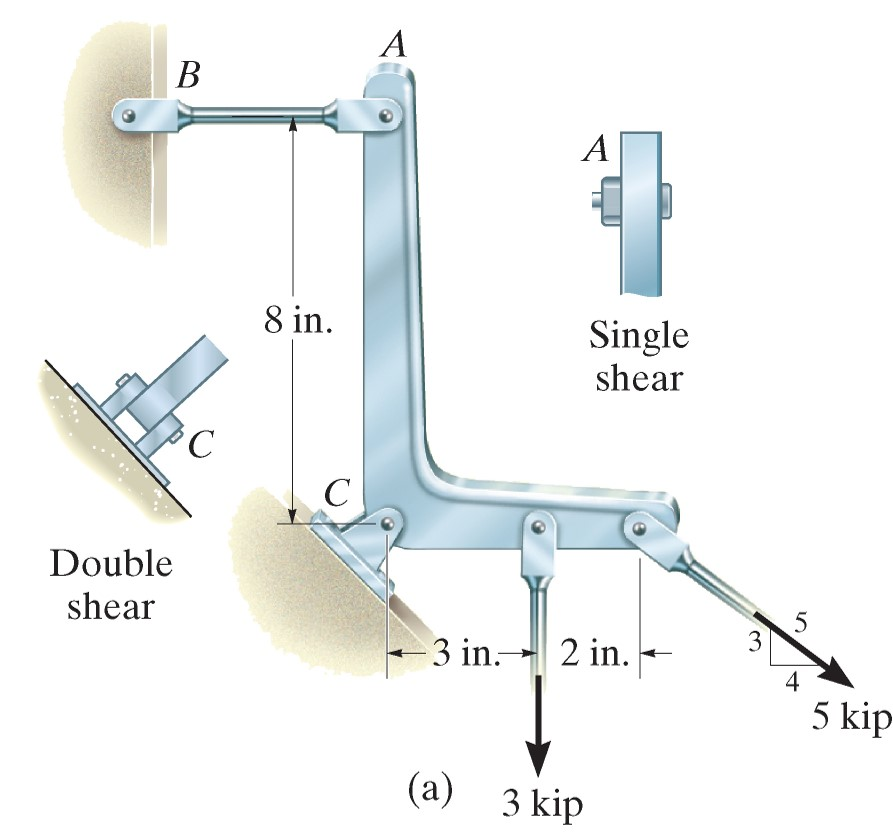
\includegraphics{../images/example-1-12.jpg}
\caption{An l-shaped bracket has an 8 inch vertical leg and a 5 inch
horizontal leg. A single shear pinned connector holds the point of the
leg, A, in place while a double shear pinned connector holds the base of
the L at point C in position. There is 3 kilopound load 3 inches to the
right of C acting downward and a 5 kilopound load 2 inches to the right
of that acting down and to the right in the direction of a 3-4-5
triangle (3 down, 4 to the right).}
\end{figure}
\end{column}

\begin{column}{0.5\textwidth}
Determine to the nearest 1/4" the diameters of steel pins at \(A\) and
\(C\) if the factor of safety in shear is 1.5 and the failure shear
stress is 12 ksi.
\end{column}
\end{columns}
\end{frame}

\begin{frame}{example 1-15}
\protect\hypertarget{example-1-15}{}
\begin{columns}[T]
\begin{column}{0.5\textwidth}
\begin{figure}
\centering
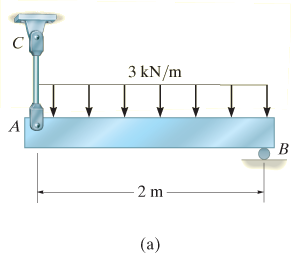
\includegraphics{../images/example-1-15.png}
\caption{A 2 meter long beam is supported at the left end with a steel
rod connecting vertically. It is subjected to a uniform load of 3
kilonewtons per meter, and a roller support at the right end.}
\end{figure}
\end{column}

\begin{column}{0.5\textwidth}
The 400 kg uniform bar, \(AB\) is supported by a steel rod \(AC\) and a
roller at \(B\). If it supports a live distributed loading, determine
the required diameter of the rod. Use \(\sigma_{fail}=345 \text{ MPa}\)
with \(\phi=0.9\), \(\gamma_D=1.2\), and \$\gamma\_L=1.6\$
\end{column}
\end{columns}
\end{frame}

\hypertarget{strain}{%
\section{strain}\label{strain}}

\begin{frame}{deformation}
\protect\hypertarget{deformation}{}
\begin{itemize}
\tightlist
\item
  When forces are applied to a body, it will change its shape and size
\item
  We call these changes \emph{deformation}
\item
  Sometimes they are barely noticeable (steel), other times they are
  very significant (rubber)
\end{itemize}
\end{frame}

\begin{frame}{strain}
\protect\hypertarget{strain-1}{}
\begin{itemize}
\tightlist
\item
  Strain is a more precise measurement of the deformation of a body
\item
  Normal strain is given as the change in length divided by the original
  length
\end{itemize}

\[\epsilon = \frac{L-L_0}{L_0}\]

\begin{itemize}
\tightlist
\item
  We can consider the average normal strain (over an entire body) or the
  local strain (take an infinitely small portion and calculate the
  strain there)
\end{itemize}
\end{frame}

\begin{frame}{units}
\protect\hypertarget{units}{}
\begin{itemize}
\tightlist
\item
  Since we divide length by length, strain is unitless
\item
  However it is customary to use \emph{in/in} or for stiff specimens to
  use the phrase \emph{microstrain} as a unit
\item
  Strain can also sometimes be represented as a percent
\end{itemize}
\end{frame}

\begin{frame}{shear strain}
\protect\hypertarget{shear-strain}{}
\begin{itemize}
\tightlist
\item
  Normal strain causes a line segment to expand or contract
\item
  Deformation can also cause two lines to change their relative angle
\item
  The change in angle between two originally perpendicular line segments
  is called shear strain
\end{itemize}

\[\gamma = \frac{\pi}{2} - \theta\]
\end{frame}

\begin{frame}{shear strain}
\protect\hypertarget{shear-strain-1}{}
\begin{figure}
\centering
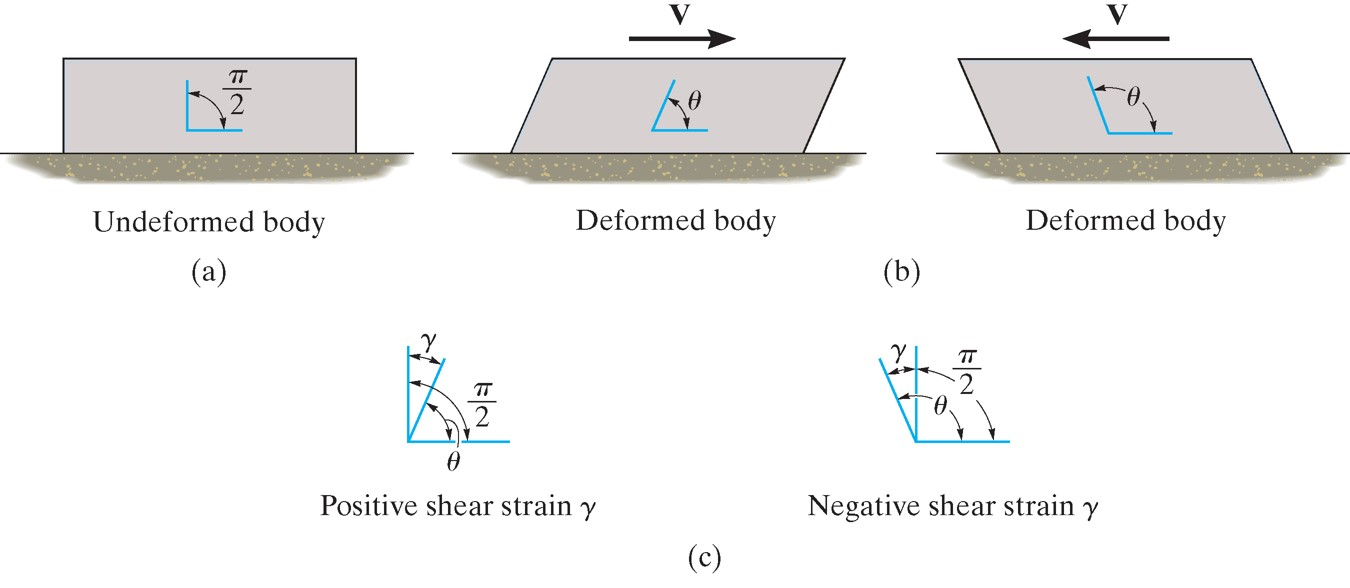
\includegraphics{../images/shear-strain.jpg}
\caption{Three stages are shown, the first is a rectangular block at
rest, with a fixed support on the ground. The second shows the block
after it deforms with a horizontal force acting along the top to the
right. The third shows the block after it deforms with a force acting
along the top to the left. The first case causes a decrease in angle
between the legs of the rectangle, the difference between 90 degrees and
the new angle is called gamma, the engineering shear strain. When the
angle becomes larger than 90 degrees, as in the third block, the
engineering shear strain is negative.}
\end{figure}
\end{frame}

\begin{frame}{cartesian components}
\protect\hypertarget{cartesian-components}{}
\begin{itemize}
\tightlist
\item
  If we consider a very small cube/prism with sides of \(\Delta x\),
  \(\Delta y\), and \(\Delta z\), normal strains will change the side
  lengths to
\end{itemize}

\[(1+\epsilon_x)\Delta x (1 + \epsilon_y)\Delta y (1 + \epsilon_z)\Delta z\]

\begin{itemize}
\tightlist
\item
  And the shear strains will change the shape
\end{itemize}

\[\frac{\pi}{2}-\gamma_{xy} \qquad \frac{\pi}{2}-\gamma_{yz} \qquad \frac{\pi}{2}-\gamma_{xz}\]
\end{frame}

\begin{frame}{small strain}
\protect\hypertarget{small-strain}{}
\begin{itemize}
\tightlist
\item
  Most engineering analysis is based on the assumption of small strains
\item
  This is valid for many materials (wood, metal), but not for rubbers
  and some other polymers
\item
  When strains are small, we assume that the change in angle,
  \(\Delta \theta\) is very small
\item
  \(\sin \Delta \theta \approx \Delta \theta\),
  \(\cos\Delta \theta \approx 1\),
  \(\tan\Delta \theta\approx \Delta \theta\)
\end{itemize}
\end{frame}

\begin{frame}{example 2.1}
\protect\hypertarget{example-2.1}{}
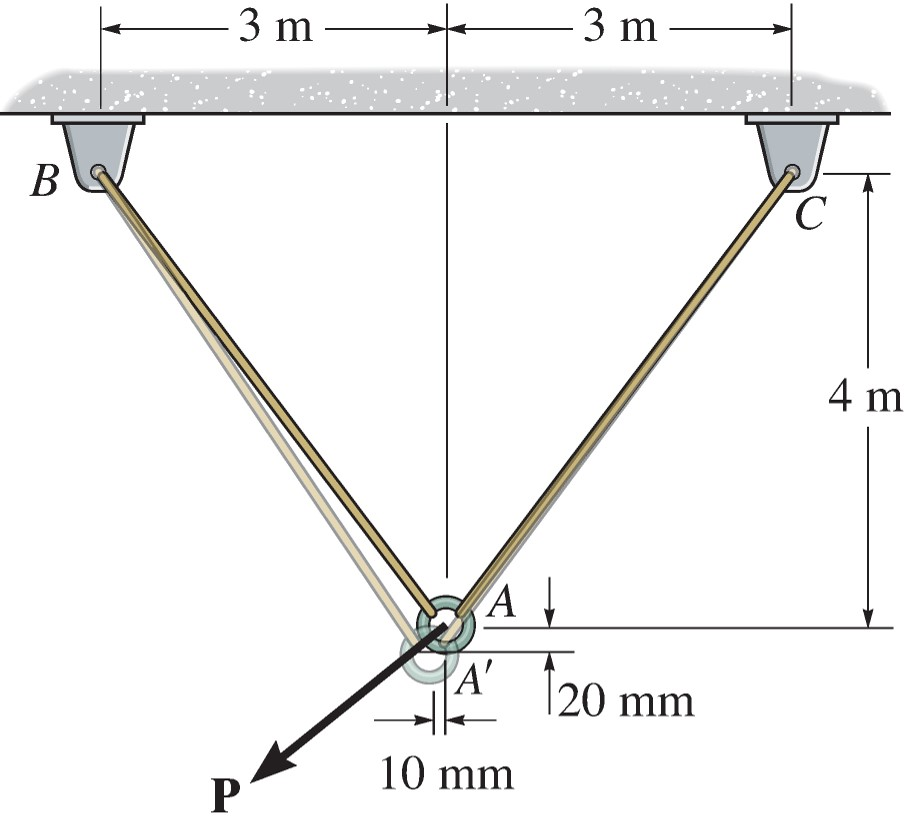
\includegraphics{../images/example-2-1.jpg}

Find the normal strains in the two wires if A moves to \(A^\prime\)
\end{frame}

\begin{frame}{example 2.3}
\protect\hypertarget{example-2.3}{}
\begin{columns}[T]
\begin{column}{0.5\textwidth}
\begin{figure}
\centering
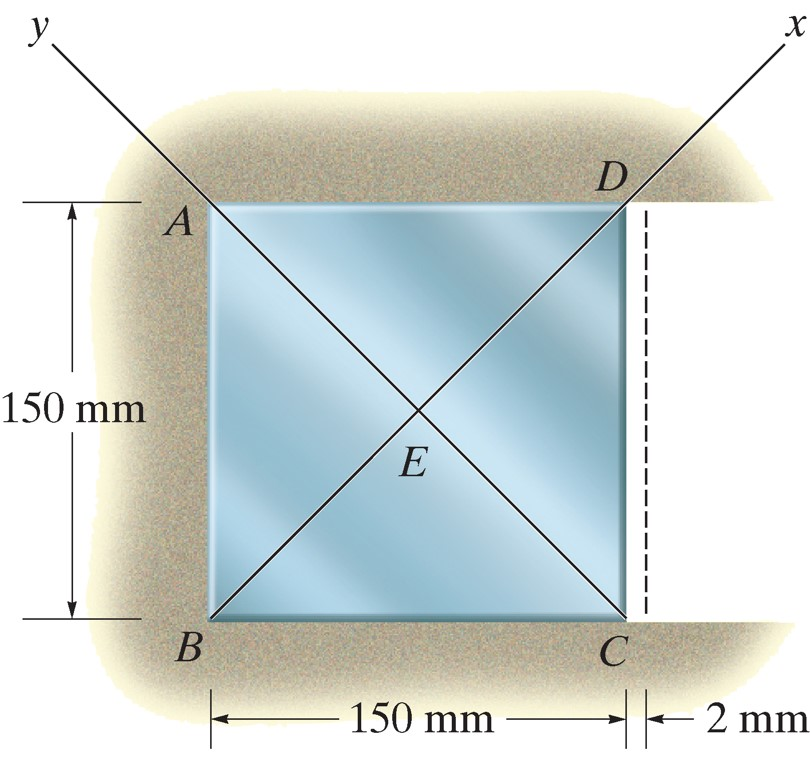
\includegraphics{../images/example-2-3.jpg}
\caption{A 150 mm square block is constrained along the top, left, and
bottom faces, but pushed 2 mm to the left on its right face. AC is the
diagonal line going from the top left to the bottom right. E is the
center point of the block (where the two diagonals intersect after
deformation).}
\end{figure}
\end{column}

\begin{column}{0.5\textwidth}
The plate is fixed along AB and held in horizontal guides along AD and
BC. If the right side is displaced 2 mm find the average normal strain
along AC and the shear strain at E relative to the x and y axes.
\end{column}
\end{columns}
\end{frame}

\end{document}
